\documentclass[8pt, landscape]{extarticle}
\usepackage[scaled=0.92]{helvet}
\usepackage{calc}
\usepackage{multicol}
\usepackage[a4paper,margin=3mm,landscape]{geometry}
\usepackage{amsmath,amsthm,amsfonts,amssymb}
\usepackage{color,graphicx,overpic}
\usepackage{hyperref}
\usepackage{newtxtext} 
\usepackage{enumitem}
\usepackage[table]{xcolor}
\usepackage{mathtools}
\usepackage{caption}
\usepackage{subfig}

\setlist{nosep}
% for including images
\graphicspath{ {./images/} }

\pdfinfo{
  /Title (CS3223.pdf)
  /Creator (TeX)
  /Producer (pdfTeX 1.40.0)
  /Author (Jovyn Tan, Jotham Wong)
  /Subject (CS3223)
/Keywords (CS3223, nus,cheatsheet,pdf)}

% Turn off header and footer
\pagestyle{empty}

% redefine section commands to use less space
\makeatletter
\renewcommand{\section}{\@startsection{section}{1}{0mm}%
  {-1ex plus -.5ex minus -.2ex}%
  {0.5ex plus .2ex}%x
{\normalfont\large\bfseries}}
\renewcommand{\subsection}{\@startsection{subsection}{2}{0mm}%
  {-1explus -.5ex minus -.2ex}%
  {0.5ex plus .2ex}%
{\normalfont\normalsize\bfseries}}
\renewcommand{\subsubsection}{\@startsection{subsubsection}{3}{0mm}%
  {-1ex plus -.5ex minus -.2ex}%
  {1ex plus .2ex}%
{\normalfont\small\bfseries}}%
\makeatother

\renewcommand{\familydefault}{\sfdefault}
\renewcommand\rmdefault{\sfdefault}
%  makes nested numbering (e.g. 1.1.1, 1.1.2, etc)
\renewcommand{\labelenumii}{\theenumii}
\renewcommand{\theenumii}{\theenumi.\arabic{enumii}.}
\renewcommand\labelitemii{•}
\renewcommand\labelitemiii{•}

\definecolor{mathblue}{cmyk}{1,.72,0,.38}
\everymath\expandafter{\the\everymath \color{mathblue}}

% Don't print section numbers
\setcounter{secnumdepth}{0}

\setlength{\parindent}{0pt}
\setlength{\parskip}{0pt plus 0.5ex}
%% adjust spacing for all itemize/enumerate
\setlength{\leftmargini}{0.5cm}
\setlength{\leftmarginii}{0.5cm}
\setlist[itemize,1]{leftmargin=2mm,labelindent=1mm,labelsep=1mm}
\setlist[itemize,2]{leftmargin=4mm,labelindent=1mm,labelsep=1mm}
\setlist[itemize,3]{leftmargin=4mm,labelindent=1mm,labelsep=1mm}

\captionsetup{belowskip=0pt}
% adding my commands
% tightcenter
\newenvironment{tightcenter}{%
  \setlength\topsep{0pt}
  \setlength\parskip{0pt}
  \begin{center}
    }{%
  \end{center}
}

% boxed
\newenvironment{tightbox}{%
  \setlength\topsep{0pt}
  \setlength\parskip{0pt}
  \begin{center}
    \begin{tabular}{|@{\hspace{\dimexpr\fboxsep+0.5\arrayrulewidth}}c@{\hspace{\dimexpr\fboxsep+0.5\arrayrulewidth}}|}
      \hline
    }
    {%
    \\ \hline
    \end{tabular}
  \end{center}
}

% fixed width box
\newenvironment{fixedbox}[1][0.7]{
  \setlength\topsep{0pt}
  \setlength\parskip{0pt}
  \begin{center}
    \begin{tabular}{|>{\centering\arraybackslash}m{#1\linewidth}|}
    \hline
  }{
  \\ \hline
  \end{tabular}
  \end{center}
}

% definition of a new term
\usepackage{soul}
\definecolor{paleyellow}{RGB}{251,243,218}
\newcommand{\definition}[2][]{\sethlcolor{paleyellow}\hl{\textbf{#2}} #1  $\rightarrow$}
% inline definition
\newcommand{\ildefinition}[1]{\sethlcolor{paleyellow}\hl{\textbf{#1}}}

% important note (attention)
\newcommand{\attention}{{\color{red}\textbf{! }}}

% nice proof
\newenvironment{niceproof}[1][Proof]
{%
  \sbox0{\textit{#1}. }%
  \list{}{\labelwidth\wd0 \leftmargin\wd0 \labelsep 0pt }
\item[\usebox0]}
  {\endlist}



% -----------------------------------------------------------------------

\begin{document}
\raggedright
\footnotesize
\begin{multicols*}{4}
  % multicol parameters
  \setlength{\columnseprule}{0.25pt}

  \begin{center}
    \fbox{%
      \parbox{0.8\linewidth}{\centering \textcolor{black}{
          {\Large\textbf{CS3223}}
        \\ \normalsize{AY22/23 SEM 2}}
        \\ {\footnotesize \textcolor{gray}{github/jovyntls github/JothamWong}}
      }%
    }
  \end{center}
  
  \begin{enumerate}
    \item k* is an actual \textbf{data record} (with search key $k$) 
    \item k* is of the form \textbf{(k, RID)} - fixed length \texttt{(k, \textbf{$\bullet$})}
    \item k* is of the form \textbf{(k, RID-list)} - e.g. (k, \{RID11, RID12\})
  \end{enumerate}

  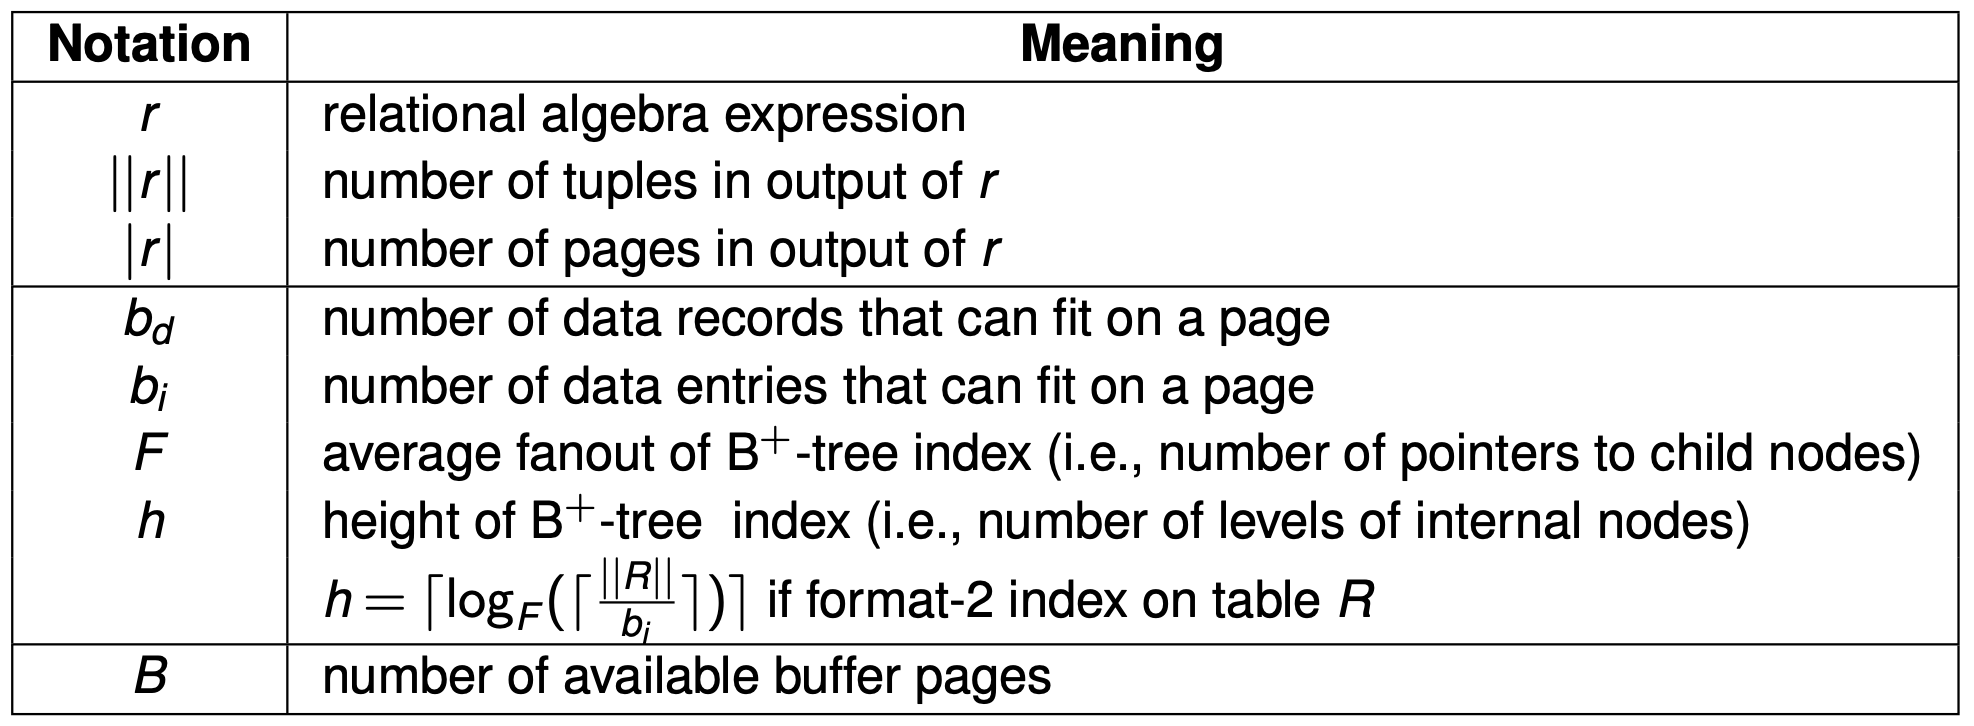
\includegraphics[width=0.95\linewidth]{cs3223-notation.png} 
  \subsection{04.1 Sorting and Selection}

  \textbf{External Merge Sort}

  \begin{itemize}
    \item \definition{sorted run} sorted data records written to a file on disk
    \item divide and conquer
      \begin{enumerate}
        \item create temporary file $R_i$ for each $B$ pages of $R$ sorted
        \item merge: use $B-1$ pages for input, 1 page for output
      \end{enumerate}
    \item total I/O = $2N(\lceil \log_{B-1}(N_0) \rceil +1)$
      \begin{itemize}
        \item $2N$ to create $\lceil N/B \rceil $ sorted runs of $B$ pages each
        \item merging sorted runs: $2N \times \lceil \log_{B-1}N_0 \rceil $
      \end{itemize}
  \end{itemize}

  \textbf{optimisation with blocked I/O}

  \begin{itemize}
    \item sequential I/O - read/write in \textit{buffer blocks} of $b$ pages
    \item one block ($b$ pages) for output, remaining blocks for input
    % \begin{minipage}[c]{0.6\linewidth}{\textcolor{black}{
      %       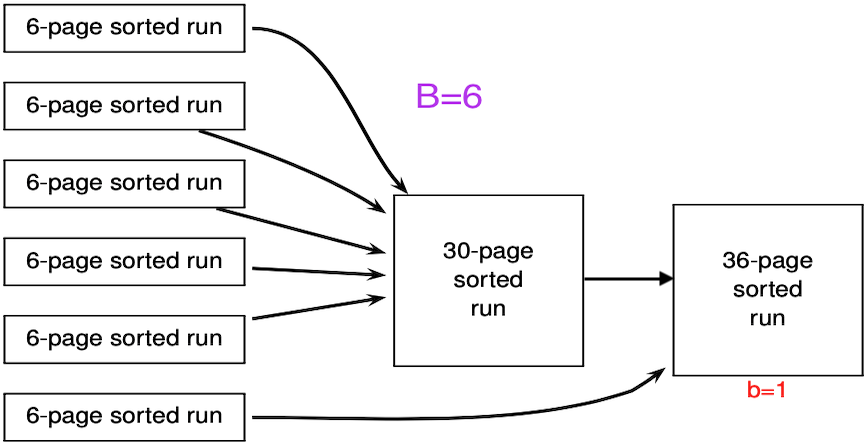
\includegraphics[width=0.97\linewidth]{cs3223-blocked-io-mergesort.png} 
  %   }}
  % \end{minipage}
    \item number of runs merged per pass, * $F = \lfloor \frac{B}{b} \rfloor -1$ 
    \item number of passes = $\lceil \log_F(N_0) \rceil +1$
  \end{itemize}
  
  \textbf{Sorting with B$^+$-trees}

  \begin{itemize}
    \item when \textit{sort key is a prefix of the index key} of the B$^+$-tree
    \item sequentially scan leaf pages of B$^+$-tree
      \begin{itemize}
        \item for Format-2/3, use RID to retrieve data records
      \end{itemize}
  \end{itemize}

  \textbf{04.2 SELECTION: $\sigma_p(R)$}

  \begin{itemize}
    \item $\sigma_p(R)$: selects rows from relation $R$ satisfying predicate $p$
    \item \textbf{access path}: a way of accessing data records/entries 
      \begin{itemize}
        \item \definition{table scan} scan all data pages
        \item \definition{index scan} scan index pages
        \item \definition{index intersection} combine results from index scans 
      \end{itemize}
    \item \definition[of an access path]{selectivity} number of index \& data pages retrieved to access data records/entries
      \begin{itemize}
        \item more selective = fewer pages retrieved
      \end{itemize}
    \item index $I$ is a \definition[for query $Q$]{covering index} if all attributes referenced in $Q$ are part of the key of $I$ 
      \begin{itemize}
        \item $Q$ can be evaluated using $I$ without any RID lookup (\ildefinition{index-only} plan)
      \end{itemize}
  \end{itemize}

  \textbf{Matching Predicates}

  \begin{itemize}
    \item \definition{term} of form $R.A \;\mathrm{op}\; c$ or $R.A_i \;\mathrm{op}\; R.A_j$
    \item \definition{conjunct} one or more terms connected by $\lor$
    \item \definition{CNF predicate} comprises one or more conjuncts connected by $\land$
      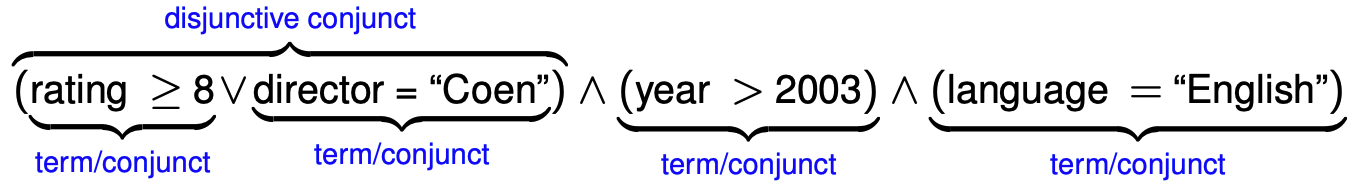
\includegraphics[width=0.80\linewidth]{cs3223-cnf-predicate.png} 
  \end{itemize}

  \textbf{B$^+$-tree matching predicates}

  \begin{itemize}
    \item for index $I=(K_1, K_2, \dots, K_n)$ and non-disjunctive CNF predicate $p$ 
      \begin{itemize}
        \item \textit{at most one} non-equality comparison operator which must be on the last attribute of the prefix ($K_i$)
      \end{itemize}
    \item matching index: matching records are in contiguous pages
      \begin{itemize}
        \item non-matching index: not contiguous $\Rightarrow$ less efficient
      \end{itemize}
  \end{itemize}

  \textbf{Hash index matching predicates}

  \begin{itemize}
    \item for hash index $I = (K_1, K_2, \dots, K_n)$ and non-disjunctive CNF predicate $p$, all attributes must be present and all ops must be equality.
  \end{itemize}

  \textbf{Primary/Covered Conjuncts}

  \begin{itemize}
    \item \definition{primary conjuncts} subset of conjuncts that $I$ matches
      \begin{itemize}
        \item e.g. $p$ = \textcolor{blue}{(age $\geq$ 18) $\land$ (age $\leq$ 20)} $\land$ (weight=65) 
          \\* for $I=$ (age, weight, height)
      \end{itemize}
    \item \definition{covered conjuncts} subset of conjuncts covered by $I$
      \begin{itemize}
        \item each attribute in covered conjuncts appears in key of $I$
      \end{itemize}
    \item primary conjuncts $\subseteq$ covered conjuncts
  \end{itemize}

  \textbf{Cost of Evaluation}

  let $p'$ = primary conjuncts of $p$, $\quad p_c$ = covered conjuncts of $p$

  \textbf{B$^+$-tree index evaluation of p}

  \begin{enumerate}
    \item navigate internal nodes to find first leaf page
      \( {\displaystyle{ 
          \text{cost}_{\text{internal}}=
          \begin{cases}
            \lceil \log_F ( \lceil \frac{||R||}{b_d} \rceil )\rceil &\text{if $$I$$ is a format-1 index}\\
            \lceil \log_F ( \lceil 
            \frac{||R||}{b_i} \rceil )\rceil  &\text{otherwise}
          \end{cases}
      }} \) 
    \item scan leaf pages to access all qualifying data entries
      \( {\displaystyle{ 
          \text{cost}_{\text{leaf}}=
          \begin{cases}
            \lceil \frac{||\sigma_{p'}(R)||}{b_d} \rceil &\text{if $$I$$ is a format-1 index}\\
            \lceil \frac{||\sigma_{p'}(R)||}{b_i} \rceil &\text{otherwise}
          \end{cases}
      }} \) 
    \item retrieve qualified data records via RID lookups
      \( {\displaystyle{ 
          \text{cost}_{\text{RID}}=
          \begin{cases}
            0 &\text{if $$I$$ is a covering format-1 index,}\\
            ||\sigma_{p_c}(R)||  &\text{otherwise}
          \end{cases}
      }} \) 
      \begin{itemize}
        \item reduce cost with \textbf{clustered} data records (sort RIDs): 
          $\lceil\frac{||\sigma_{p_c}(R)||}{b_d}\rceil \leq \text{cost}_{RID} \leq \min\{||\sigma_{p_c}(R)||, |R|\}$
      \end{itemize}
  \end{enumerate}

  \textbf{hash index evaluation of p}

  \begin{itemize}
    \item \textbf{format-1}: $\quad$ cost to retrieve data records $ \geq \lceil\frac{||\sigma_{p'}(R)||}{b_d}\rceil $
    \item \textbf{format-2}: $\quad$ cost to retrieve data entries $ \geq \lceil\frac{||\sigma_{p'}(R)||}{b_i}\rceil $ 
      \\* cost to retrieve data records = $ \begin{cases} 0 \quad \text{if $$I$$ is a covering index,}\\
        ||\sigma_{p'}(R)||  \quad \text{otherwise}
      \end{cases} $
  \end{itemize}


  \subsection{05. PROJECTION $\pi_{A_1, \dots, A_m}(R)$ AND JOIN}

  \begin{itemize}
    \item $\pi_L(R)$ eliminates duplicates, $\pi^*_L(R)$ preserves duplicates
  \end{itemize}

  \textbf{Sort-based approach}

  % 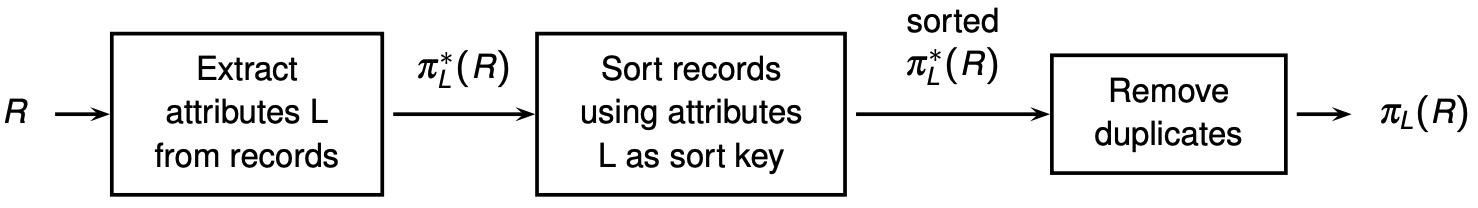
\includegraphics[width=0.95\linewidth]{cs3223-projection-sort-approach.png} 

  \textbf{cost analysis}

  \begin{enumerate}
    \item extract attributes: $|R|$ scan + $\vert \pi^*_L(R)\vert$ output temp result
    \item sort records: $2\vert \pi^*_L(R) \vert (\log_m(N_0) +1)$
    \item remove duplicates: $\vert \pi^*_L(R)\vert$ to scan records
  \end{enumerate}

  \textbf{optimised sort-based approach}

  % 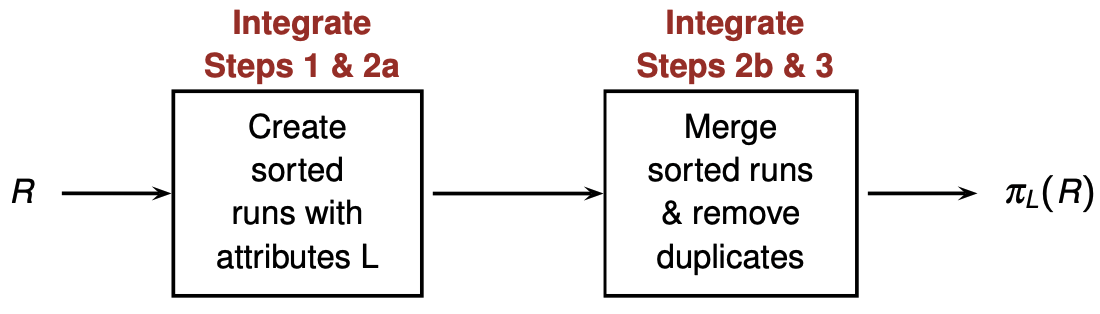
\includegraphics[width=0.8\linewidth]{cs3223-projection-sort-approach-optimised.png} 

  \begin{itemize}
    \item if $B>\sqrt{|\pi^*_L(R)|}$, same I/O cost as hash-based approach
      \begin{itemize}
        \item $N_0 = \lfloor \frac{|R|}{B} \rfloor \approx \sqrt{|\pi^*_L(R)|}$ initial sorted runs 
        \item $\log_{B-1}(N_0) \approx 1$ merge passes
      \end{itemize}
  \end{itemize}

  \textbf{Hash-based approach}

  \begin{enumerate}
    \item \textbf{partitioning phase}: hash each tuple $t \in R$ 
      \begin{itemize}
        \item $R = R_1 \cup R_2 \cup \dots \cup R_{B-1}$
          \begin{itemize}
            \item for each $R_i$ \& $R_j$, $i \neq j$, $\pi_L^*(R_i) \cap \pi_L^*(R_j) = \emptyset$
          \end{itemize}
        \item for each $t$: project attributes to form $t'$, hash $h(t')$ to one output buffer, flush output buffer to disk when full
        \item one buffer for input, $(B-1)$ buffers for output
      \end{itemize}
    \item \textbf{duplicate elimination} from each $\pi^*_L(R_i)$
      \begin{itemize}
        \item for each $R_i$: initialise in-mem hash table, hash each $t \in R_i$ to bucket $B_j$ with $h' \neq h$, insert if $t \not\in B_j$
        \item write tuples in hash table to results
      \end{itemize}
  \end{enumerate}
  % 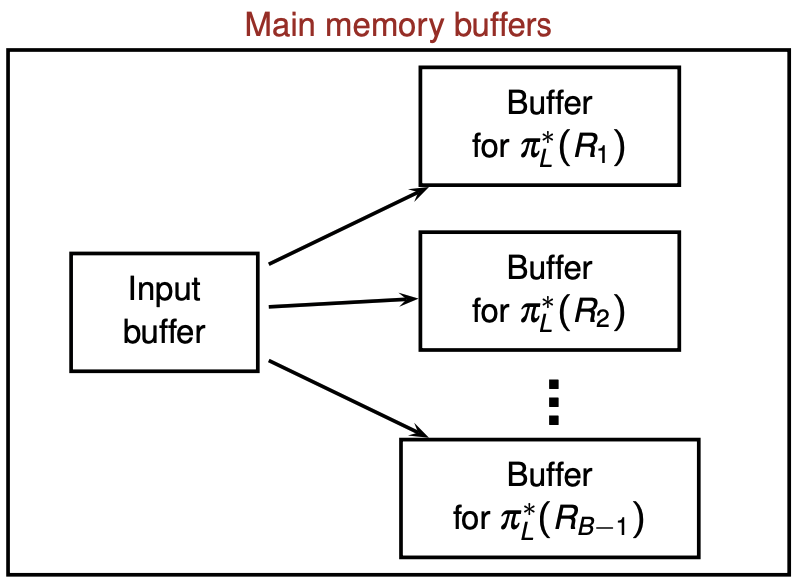
\includegraphics[width=0.4\linewidth]{cs3223-projection-hash-1.png} 
  % 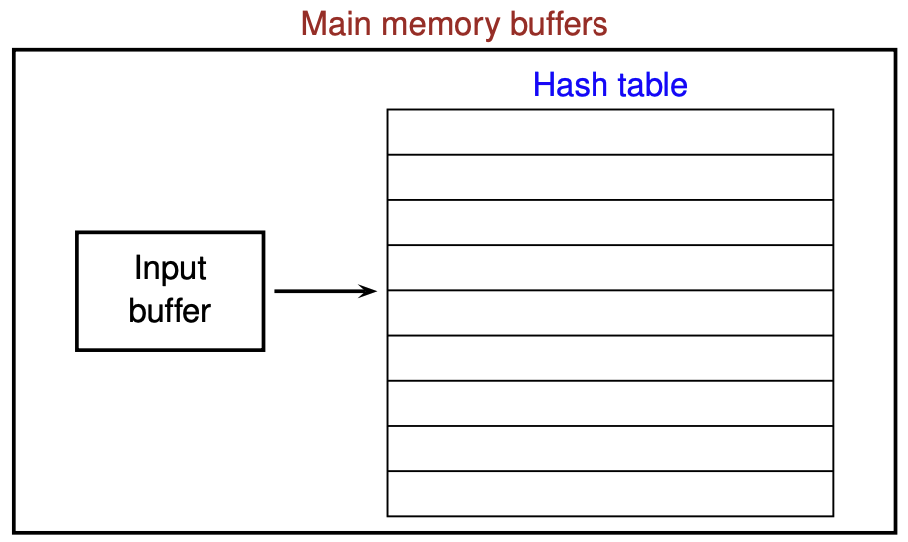
\includegraphics[width=0.5\linewidth]{cs3223-projection-hash-2.png} 

  \begin{itemize}
    \item \textbf{I/O cost} (no partition overflow): $|R| + 2|\pi^*_L(R)|$
      \begin{itemize}
        \item partitioning cost: $|R| + |\pi^*_L(R)|$
        \item duplicate elimination cost: $|\pi^*_L(R)|$
      \end{itemize}
    \item partition overflow: recursively apply partitioning
      \begin{itemize}
        \item to avoid, $B>$ size of hash table for $R_i$ = $\frac{|\pi^*_L(R)|}{B_1} \times f$
          \begin{itemize}
            \item  approximately $B> \sqrt{f\times |\pi^*_L(R)|}$
          \end{itemize}
          % 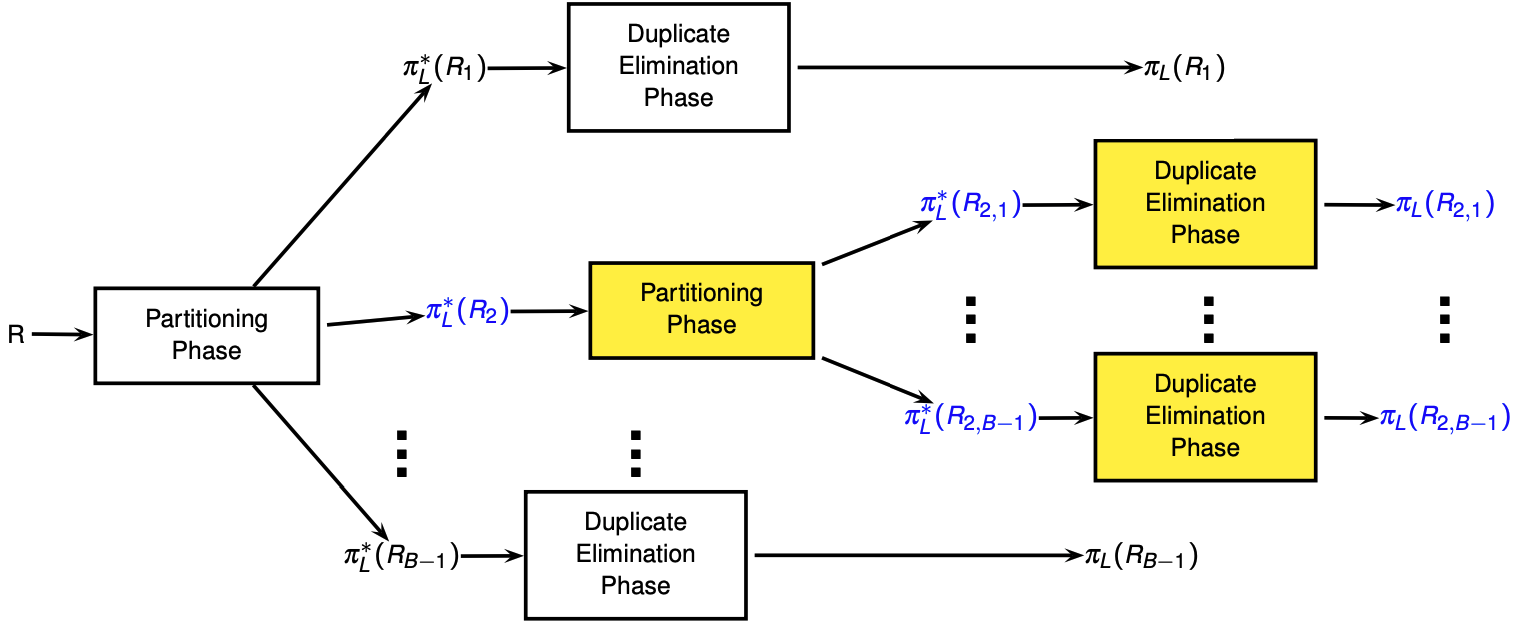
\includegraphics[width=0.9\linewidth]{cs3223-projection-hash-partition-overflow.png} 
      \end{itemize}
  \end{itemize}

  \textbf{Projection using Indexes}

  \begin{itemize}
    \item if index search key contains all wanted attributes \textit{as a prefix}
      \begin{itemize}
        \item \textbf{index scan} data entries in order \& eliminate duplicates
      \end{itemize}
  \end{itemize}

  \textbf{05.2 JOIN $R \bowtie_\theta S$}

  $R$ = outer relation (smaller relation); $\quad S$ = inner relation

  \attention for \textbf{format-2} index, add cost of retrieving record

  \textbf{nested loop joins}

  \begin{itemize}
    \item \textbf{tuple-based} nested loop join: $|R| + ||R|| \times |S|$
    \item \textbf{page-based} nested loop join: $|R| + |R| \times |S|$
    \item \textbf{block nested loop join}: $|R| + ( \lceil \frac{|R|}{B-2} \rceil \times |S| )$, $\;\; |R|\leq|S|$
      \begin{itemize}
        \item 1 page output, 1 page input, $(B-2)$ pages to read $R$
        \item for each $(B-2)$ pages of $R$: for each $P_S$ of $S$: check r,s
      \end{itemize}
    \item \textbf{index nested loop join}: $|R| + ||R|| \times \left( \log_F(\lceil \frac{||S||}{b_d} \rceil ) + \lceil \frac{||S||}{b_d ||\pi_{B_j}(S)||} \rceil \right)$
      \begin{itemize}
        \item joining $R(A, B) \bowtie_A S(A,C)$ with B+tree index on $S.A$
        \item for each tuple $r \in R$, use $r$ to probe $S$'s index for match
      \end{itemize}
  \end{itemize}

  \textbf{sort-merge join}

  \begin{itemize}
    \item sort R \& S: $2|R| (\log_m(N_R)+1) + 2|S| (\log_m(N_S)+1)$
    \item merge cost: $|R| + |S| \quad$ (worst case $|R| + ||R||\times|S|$)
  \end{itemize}

  \textbf{optimised sort-merge join}

  \begin{itemize}
    \item merge sorted runs until $B > N(R, i) + N(S, j)$; then do merge and join at the same time
    \item I/O cost: $3 \times (|R|+|S|)$
      \begin{itemize}
        \item if $B > \sqrt{2|S|}$, one pass to merge initial sorted runs
        \item $2(|R|+|S|)$ for initial sorted runs, $|R|+|S|$ for merging
      \end{itemize}
  \end{itemize}

  \textbf{hash join}

  \begin{enumerate}
    \item partition $R$ and $S$ into $k$ partitions on join column
      \begin{itemize}
        \item $\pi_A(R_i) \cap \pi_B(S_j) = \emptyset \quad \forall R_i, S_j, i \neq j$
        \item $R = R_1 \cup R_2 \cup \dots \cup R_k, \quad t \in R_i \iff h(t.A)=i$
        \item $S = S_1 \cup S_2 \cup \dots \cup S_k, \quad t \in S_i \iff h(t.B)=i$
      \end{itemize}
    \item join corresponding partitions: $R \bowtie_{R.A=S.B} S = (R_1 \bowtie S_1) \cup \dots \cup (R_k \bowtie S_k)$
  \end{enumerate}

  \textbf{Grace hash join}

  for \textit{build relation} $R$ and \textit{probe relation} $S$,
  \begin{enumerate}
    \item \textbf{partition} $R$ and $S$ into  $k$ partitions each, $k=B-1$
    \item \textbf{probing phase}: hash $r \in R_i$ with $h'(r.A)$ to table $T$
      \begin{enumerate}
        \item $\forall s \in S_i$, $r \in$ bucket $h'(s.B)$: output ($r,s$) if match
      \end{enumerate}
  \end{enumerate}

  \begin{itemize}
    \item I/O cost: $3(|R|+|S|) \quad$ (no partition overflow)
    \item $B > \frac{f \times |R|}{B-1} + 2$ (input \& output buffer) $\approx B > \sqrt{f\times |R|}$
      \begin{itemize}
        \item during probing, $B >$ size of each partition $+ 2$
      \end{itemize}
    \item \textbf{partition overflow} if $R_i$ cannot fit in memory
      \begin{itemize}
        \item recursively apply partitioning to overflow partition
      \end{itemize}
  \end{itemize}

  \textbf{General join conditions}

  \begin{itemize}
    \item \textbf{multiple equality-join} conditions: $(R.A = S.A) \land (R.B=S.B)$
      \begin{itemize}
        \item index nested loop join: use index on some/all join attribs
        \item sort-merge join: sort on \textit{combination} of attributes
        \item other algos: no change
      \end{itemize}
    \item \textbf{inequality-join} conditions: $(R.A<S.A)$
      \begin{itemize}
        \item index nested loop join: requires B$^+$-tree index
        \item not applicable: sort-merge join (too much rewinding), hash-based joins
        \item other algos: no change
      \end{itemize}
  \end{itemize}

  \subsection{06. Query Evaluation \& Optimization}

  \begin{itemize}
    \item Set operations can be implemented with joins and sort/hash
    \begin{itemize}
      \item $R(A, B) \cap S(A, B) = \pi_{R.A, R.B} R \bowtie_{p} S$
      \item where p = (R.A = S.A) $\wedge$ (R.B = S.B)
    \end{itemize}
    \item Sorting for $R \cup S$
    \begin{itemize}
      \item Sort R and S using all attributes. Merge the sorted operands.
    \end{itemize}
    \item Hashing for $R \cup S$
    \begin{itemize}
      \item Same as grace hash join, k partitions, when probing, discard if in, else add. Write to disk.
    \end{itemize}
    \item Aggregation: maintain running info while scanning table.
    \begin{itemize}
      \item Use index scan on covering index whenever possible.
    \end{itemize}
    \item Group by: Partition by grp attr and run normal aggregation.
    \item \textbf{Materialized evaluation}
    \begin{itemize}
      \item Evaluate operator only when all operands are evaluated or materialized.
      \item Intermediate results are written to disk which can be costly.
    \end{itemize}
    \item \textbf{Pipelined evaluation}
    \begin{itemize}
      \item Execution of operators is interleaved. Pipelining may not always be possible. 
      \item Temporary relations are not stored on disk.
      \item Output produced by operator is passed directly to parent.
      \item \textbf{Blocking operator} O cannot start until all receive all input tuples from children operators
      \item Examples are external merge sort, smj, grace hash.
      \item Use \textbf{partial materialization} cheaper to read from temp output relation (due to very selective p)
      \item Iterator interface.
      \begin{itemize}
        \item \textbf{open}: initialize iterator state: resources, args.
        \item \textbf{getNext}: gen next tuple, return null when done
        \item \textbf{close}: Deallocate state information
      \end{itemize}
    \end{itemize}
    \item A SQL query has many equiv logical plans, which have many equiv physical plans
    \item Query optimization is about avoiding the worst plans, not picking the best
    \item Relational Algebra Equiv rules
  \end{itemize}
    \begin{enumerate}
      \item Commutativity of binary ops
      \begin{enumerate}
        \item $R \times S \equiv S \times R$
        \item $R \bowtie S \equiv S \bowtie R$ 
      \end{enumerate}
      \item Associativity of binary ops
      \begin{enumerate}
        \item $(R \times S) \times T \equiv R \times (S \times T)$
        \item $(R \bowtie S) \bowtie T \equiv R \bowtie (S \bowtie T)$
      \end{enumerate}
      \item Idempotence of unary op
      \begin{enumerate}
        \item $\pi_{L'}(\pi_{L}(R)) \equiv \pi_{L'}(R)$ if $L' \subseteq L \subseteq attr(R)$
        \item $\sigma_{p1}(\sigma_{p2}(R)) \equiv \sigma_{p1 \wedge p2}(R)$
      \end{enumerate}
      \item Commutating selection with projection
      \begin{enumerate}
        \item $\pi_L(\sigma_p(R)) \equiv \pi_L(\sigma_p(\pi_{L \cup attr(p)}(R)))$
      \end{enumerate}
      \item Commutating selection with binary ops
      \begin{enumerate}
        \item $\sigma_p(R \times S) \equiv \sigma_p(R) \times S$
        \item $\sigma_p(R \bowtie_{p'} S) \equiv \sigma_p(R) \bowtie_{p'} S$
        \item assuming $attr(p) \subseteq attr(R)$
        \item $\sigma_p(R \cup S) \equiv \sigma_p(R) \cup \sigma_p(S)$
      \end{enumerate}
      \item Commutating proj with binary ops\\Let $L = L_R \cup L_S$ where $L_R \subseteq attr(R), L_S \subseteq attr(S)$
      \begin{enumerate}
        \item $\pi_L(R \times S) \equiv \pi_{L_R}(R) \times \pi_{L_S}(S)$
        \item $\pi_L(R \bowtie_p S) \equiv \pi_{L_R}(R) \bowtie_p \pi_{L_S}(S)$\\if attr(p) $\cap$ attr(R) $\subseteq$ $L_R$ and attr(p) $\cap$ attr(S) $\subseteq$ $L_S$ 
        \item $\pi_L(R \cup S) \equiv \pi_L (R) \cup \pi_L (S)$
      \end{enumerate}
    \end{enumerate}
    \begin{itemize}
      \item Summary of RA optimization
      \begin{enumerate}
        \item Perform selection as early as possible, ideally before joins.
        \item Replace Cartesian Product by join whenever possible
        \item Project out useless attributes early
        \item If there are several joins, perform most restrictive join first.
      \end{enumerate}
      \item Types of Query Plan Trees
      \begin{itemize}
        \item A query plan is \textbf{linear} if at least one operand for each join op is a base relation, else it is \textbf{bushy}
        \item A linear plan is \textbf{left-deep} if every right operand is a base relation
        \item A linear plan is \textbf{right-deep} if every left operand is a base relation
      \end{itemize}  
      \item Query plan enumeration, assume that optimal sol to smaller set is optimal sol to larger set. may not be true.
      \item DP algorithm for query enumeration: Calculate optimal plan for all single relations. Calculate optimal plan involving 2, 3 and so on relations by finding best way to join each smaller relation.
      \item System R optimizer
      \begin{itemize}
        \item Enumerate only left-deep query plans. (too much to search o/w)
        \item Avoid cross-product query plans.
        \item Consider early selections and projections.
        \item Uses $dp(S_i, o_i)$ where $o_i$ is null if unordered or a sequence of attrs
        \item May be cheaper if a SMJ is sorted on some sequence even if by itself is suboptimal. 
      \end{itemize}
      \item Cost estimation
      \begin{itemize}
        \item Uniformity assumption: uniform distribution
        \item Independence assumption: diff attrs are independent
        \item Inclusion assumption: For $R \bowtie_{R.A = S.B} S$, if $\lVert{\pi_A (R)}\lVert \leq \lVert{\pi_B (S)}\lVert$ then $\pi_A (R) \subseteq \pi_B(S)$
      \end{itemize}
      \item \textbf{Size estimation}: $\lVert q \lVert \approx \lVert e \lVert \times \prod_{i=1}^{n}rf(t_i)$
      \begin{itemize}
        \item $rf(t_i) = \frac{\lVert \sigma_i(e)\lVert}{\lVert e \lVert}$, reduction/selectivity factor
        \item $rf(R=c) = \frac{\lVert c \lVert}{\lVert R \lVert}$ uniformity assumption
      \end{itemize}
      \item \textbf{Join selectivity}: $rf(R.A = S.B) = \frac{\lVert R \bowtie_{R.A = S.B} \lVert}{\lVert R \lVert \times \lVert S \lVert}$
      \begin{itemize}
        \item Inclusion assumption: Assume that $\lVert \pi_A(R) \lVert \leq \lVert \pi_B(S) \lVert$
        \item By uniformity assumption, every R-tuple joins with $\frac{\lVert S \lVert}{\lVert \pi_B(S) \lVert}$
        \item $\therefore rf(R.A = S.B) \approx \frac{1}{\max(\lVert \pi_A(R) \lVert, \lVert \pi_B(S) \lVert)}$ 
      \end{itemize}
      \item Using histograms. Partition domain into sub-ranges (\textbf{buckets}) and assume uniform value distribution within each bucket.
      \begin{itemize}
        \item \textbf{Equiwidth}: Each bucket has almost equal num values
        \item \textbf{Equidepth}: Each bucket has almost equal num tuples, sub-range of adj buckets can overlap
        \item \textbf{MCV}: Keep track of exact top-k common values and exclude from buckets 
      \end{itemize}
    \end{itemize}
  \subsection{07. Transaction}

  \begin{itemize}
    \item An active Xact is a Xact still in progress
    \item \textbf{Schedule} = A list of actions from a set of Xacts where the order of the actions within each Xact is preserved
    \item \textbf{Serial Schedule} = A schedule where the actions of Xacts are not interleaved
    \item We say that \textbf{$T_j$ reads O from $T_i$} in a schedule S if the last write on O before $R_j(O)$ in S is $W_i(O)$ 
    \item We say that $T_j$ reads $T_i$ if $T_j$ has read some object from $T_i$ 
    \item We say that $T_i$ performs the final write on $O$ in a schedule S if the last write on O is $W_i(O)$
    \item An interleaved Xact schedule is \textbf{correct} if it is "equivalent" to some serial schedule over the set of Xacts 
  \end{itemize}
  
  Two schedules $S$ and $S'$ (over the same set of Xacts) are \textbf{view equivalent} denoted by $S \equiv_v S'$ if they satisfy:

  \begin{enumerate}
    \item If $T_i$ reads $A$ from $T_j$ in S, then $T_i$ must also read $A$ from $T_j$ in $S'$
    \item For each data object $A$, the Xact (if any) that performs the final write on $A$ in $S$ must also perform the final write on $A$ in $S'$
  \end{enumerate}

  A schedule S is a \textbf{view serializable schedule (VS)} if S is view equivalent to some serial schedule over the same set of Xacts

  We can also construct a directed VSG(S) to capture read-from and final-write relations among Txn. Each node in VSG repr a Txn with the following edges
  \begin{enumerate}
    \item $(T_j, T_i)$ if $T_i$ reads from $T_j$
    \item $(T_j, T_i)$ if both $T_i$ and $T_j$ update the same O and $T_i$ does final write on O
    \item $(T_j, T_i)$ if $T_j$ read O from initial db and $T_i$ update O
  \end{enumerate}
  If VSG(S) is cyclic, then S is not VSS. If VSG(S) is acylic, then S is VSS iff there exists a serial schedule produced from a topo ordering of VSG(S) that is view equivalent to S.

  Two actions on the same O \textbf{conflict} if at least one is a W and both are from diff Xacts
  
  \begin{enumerate}
    \item Dirty read (due to WR conflicts)
    \begin{itemize}
      \item $T_2$ reads O modified by $T_1$ and $T_1$ has not yet committed.
      \item $W_1(x), R_2(x)$
      \item $T_2$ can see an inconsistent DB state 
    \end{itemize}
    \item Unrepeatable read (due to RW conflicts)
    \begin{itemize}
      \item $T_2$ updates O that $T_1$ reads and $T_2$ commits while $T_1$ is still in progress
      \item $R_1(x), W_2(x), \text{Commit}_2, R_1(x)$
      \item $T_1$ can get a different value if it reads O again
    \end{itemize} 
    \item Lost update (due to WW conflicts)
    \begin{itemize}
      \item $T_2$ overwrites O that was modified by $T_1$ while $T_1$ is still in progress
      \item $R_1(x), R_2(x), W_1(x), W_2(x)$
      \item $T_1$'s update is lost
    \end{itemize}
    \item Phantom read
    \begin{itemize}
      \item T re-executes a query on a predicate and gets a different set of results due to a recently commited T.
      \item Can be prevented by \textbf{predicate locking}: Grant T an S on p, another T' request for X on p is blocked. Also see \textbf{index locking}
    \end{itemize}
  \end{enumerate}

  \begin{itemize}
    \item \textbf{conflict equivalent} denoted by $S \equiv_c S'$ if they order every pair of conflicting actions of two \textbf{committed} Xacts in the same way.
    \item \textbf{conflict serializable schedule (CS)} if it is conflict equivalent to a serial schedule over the same set of Xacts.
    \item \textbf{Conflict serializability graph} denoted as $\text{CSG(S)} = (V, E)$ s.t
    \begin{itemize}
      \item $V$ contains a node for each committed Xact in $S$
      \item $E$ contains $T_i, T_j$ if an action in $T_i$ precedes and conflicts with one of $T_j$'s action.
    \end{itemize}
    \item \textbf{Theorem}: A schedule is \textbf{CS} iff its $\text{CSG}$ is acyclic.
    \item \textbf{Theorem}: $CSS \subsetneq VSS \subsetneq MVSS$.
    \item \textbf{Note}: CS3223 uses \textbf{serializable} to mean \textbf{CS}
    \item A write on O by $T_i$ is a \textbf{blind write} if $T_i$ did not read O prior to the write
    \item \textbf{Theorem}: If S is \textbf{VS} and S has no blind writes, then S is also \textbf{CS}.
  \end{itemize}

  \begin{itemize}
    \item \textbf{Cascading abort}: For correctness, if $T_i$ read from $T_j$ then $T_i$ must abort if $T_j$ aborts. We say that $T_j$'s abort is cascaded to $T_i$.
    \item \textbf{Recoverable schedule}: For every Xact T that commits in S, $T$ must commit after $T'$ if $T$ reads from $T'$.
    \item Recoverable schedules guarantee that committed Xacts will not be aborted but cascading aborts of active Xacts are possible.
    \item \textbf{Cascadeless schedule}: If whenever $T_i$ reads from $T_j$ in S, $\text{Commit}_j$ must precede this read action.
    \item \textbf{Theorem}: A cascadeless schedule is recoverable.
    \item \textbf{Before-images}: Log the before-images of writes to undo the aborted Xacts. See Chap 10. But this does not always work.
    \begin{itemize}
      \item $W_1(A), W_2(A), \text{Abort}_1$. Undoing $W_1(A)$ is incorrect.
    \end{itemize} 
    \item \textbf{Strict}: For every $W_i(O)$ in S, O is not read or written by another Xact until $T_i$ either aborts or commits.
    \begin{itemize}
      \item Recovery using before-images is more efficient.
      \item Concurrent executions are more restrictive.
    \end{itemize}
    \item \textbf{Theorem}: $\text{Strict} \subsetneq \text{Cascadeless} \subsetneq \text{Recoverable}$.
  \end{itemize}

  \subsection{08. Concurrency Control}
  \textbf{Transaction Scheduler}: For each input action (R, W, C, A) to the scheduler, either output action to S, postpone(block Xact) or reject (abort Xact)

  \textbf{Lock-Based concurrency control}
  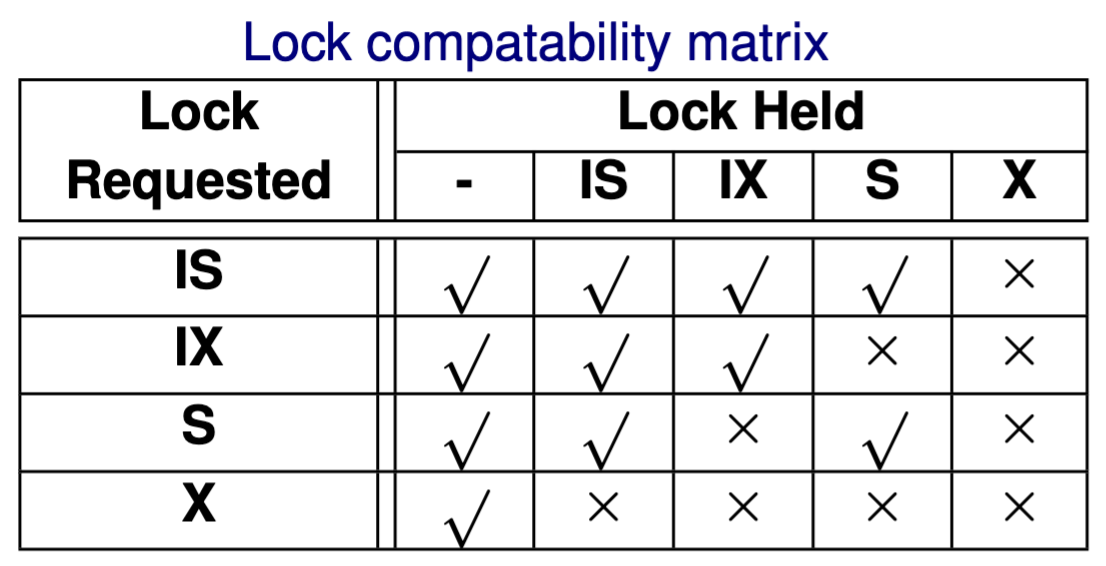
\includegraphics[width=0.4\linewidth]{cs3223-lock-matrix.png}
  \begin{enumerate}
    \item If lock request not granted, T becomes \textbf{blocked}, execution is suspended and T is added to O's request queue.
    \item When a lock on O is released, lock manager checks request of first T in request queue for O. If can be granted, T acquires lock on O and resumes after popped from queue.
    \item When an Xact commits/aborts, all locks are released and T is removed from any request queue it's in.
    \item $S_i(O):$ Xact $T_i$ requests S on O
    \item $X_i(O):$ Xact $T_i$ requests X on O
    \item $U_i(O):$ Xact $T_i$ releases lock on O
  \end{enumerate}

  \textbf{Two Phase Locking (2PL) Protocol}
  \begin{enumerate}
    \item To read O, T must hold S or X on O.
    \item To write O, T must hold X on O.
    \item Once T releases a lock, T cannot request anymore.
    \item 2PL = growing and shrinking phase.
    \item \textbf{Theorem:} 2PL S are CS.
  \end{enumerate}

  \textbf{Strict 2PL}
  \begin{itemize}
    \item Same as 2PL points 1 and 2.
    \item T must hold onto locks until T commits or aborts.
    \item \textbf{Theorem:} Strict 2PL S are strict and CS.
  \end{itemize}

  \begin{itemize}
    \item \textbf{Deadlock Detection: Waits-for graph (WFG)}
    \begin{itemize}
      \item Nodes represent active T.
      \item Add edge $T_i \rightarrow T_j$ if $T_i$ waiting for $T_j$ to release lock.
      \item Remove edge when lock request is granted.
    \end{itemize}
    \item Deadlock detected if WFG has a cycle.
    \item Break deadlock by aborting a T in the cycle.
    \item Alternative: timeout.
  \end{itemize}
  \begin{itemize}
    \item \textbf{Deadlock Prevention}: Older T have higher priority than younger T
    \begin{itemize}
      \item Each T is assigned ts when started. Older T has a smaller ts.
    \end{itemize}
    \item Suppose $T_i$ requests for a lock that conflicts with a lock held by $T_j$
    \item 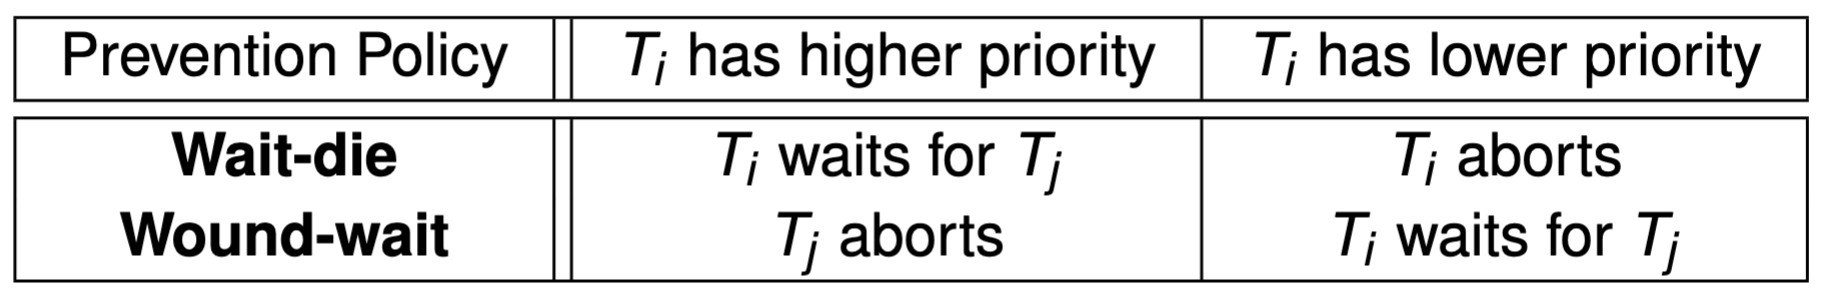
\includegraphics[width=0.15\textwidth]{cs3223-deadlock-prevention.png}
    \item Wait-die policy
    \begin{itemize}
      \item non-preemptive: only requesting T can be aborted
      \item younger T may abort repeatedly
      \item T that has all locks is never aborted
    \end{itemize}
    \item Wound-wait policy is preemptive
    \item To avoid starvation, a restarted T must use original timestamp
  \end{itemize}

  \textbf{Lock Conversion} Increases concurrency by allowing lock conversions, previously serial only schedules can become interleaved.
  \begin{itemize}
    \item $\text{UG}_i(A):$ $T_i$ upgrades S on A to X.
    \begin{itemize}
      \item Blocked if another T is holding S on A.
      \item Allowed if $T_i$ has not released any lock.
    \end{itemize}
    \item $\text{DG}_i(A):$ $T_i$ downgrades X on A to S.
    \begin{itemize}
      \item Allowed if $T_i$ has not modified A and $T_i$ has not released any lock.
    \end{itemize}
  \end{itemize}

  \textbf{Lock-based Isolation levels}

  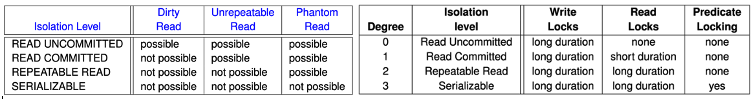
\includegraphics[width=0.2486\textwidth]{cs3223-isolation-levels.png} 
  \begin{itemize}
    \item \textbf{Short duration} lock acquired for an operation can be released after operation ends before T commits/abort
    \item \textbf{Long duration} lock acquired for an operation is held until T commits/abort
    \item \textbf{Lock Granularity}: Highest(coarsest) to lowest(finest): db, relation, page, tuple
    \item If T holds M on D, T implicitly holds M on granules finer than D.
    \item \textbf{Protocol}: Before acquiring S/X on G, acquire IS/IX on granules coarser than G top-down. Release locks bottom-up.
  \end{itemize}

  \subsection{09. MVCC}
  \begin{itemize}
    \item $W_i(O_i): $ create new version of O denoted by $O_i$. $O_0$ is initial version.
    \item $R_i(O_j): $ read an appropriate version of O
    \item Read-only T not blocked by update T and vice versa
    \item Read-only T never aborted
  \end{itemize}

  \begin{itemize}
    \item \textbf{Multiversion view equivalent (MVE)} denoted by $S \equiv_{mv} S'$ if they have the same set of reads-from.
    \item $R_i(x_j)$ occurs in S iff $R_i(x_j)$ also occurs in S'
    \item \textbf{Monoversion schedule}: each read in S returns most recently created version. Also can be serial.
    \item \textbf{Multiversion view serializable s (MVSS)}: a S where there exists a serial monoversion S' that is MVE to S.
    \item To show not MVSS, suppose there exists a S' and show that there is a cycle in the precede graph.
  \end{itemize}

  \begin{itemize}
    \item \textbf{MVCC Protocol: Snapshot Isolation (SI)}
    \item Each T has two timestamps $start(T)$ and $commit(T)$
    \item Each T sees a snapshot of DB that consists of updates by T' that committed before T starts
    \item T and T' are \textbf{concurrent} if they overlap
    \item $O_i$ is a \textbf{newer version} compared to $O_j$ if $\text{commit}(T_i) > \text{commit}(T_j)$
    \item If $R_i(O)$ returns $O_j$ then (either own update or latest version of O created by T that committed before $T_i$ starts)
    \begin{itemize}
      \item $j = i$ if $W_i(O)$ precedes $R_i(O)$ OR
      \item $\text{commit}(T_j) < \text{start}(T_i)$
      \item For every $T_k$, $k \neq j$, that has created a version $O_k$ of O if $\text{commit}(T_k) < \text{start}(T_i) \text{then} \text{commit}(T_k) < \text{commit}(T_j)$ 
    \end{itemize}
    \item \textbf{Concurrent update property:} If multiple concurrent T updated same O, only one T allowed to commit. If not, S may not be serializable.
    \item \textbf{First Committer Wins (FCW)}: Before committing T, if another committed concurrent T' that has updated some O that T has updated exists, abort T. Else commit T.
    \item \textbf{First Updater Wins (FUW)}: When T needs to update O, T requests for X. If X is not held by another concurrent T'
    \begin{itemize}
      \item T is granted X on O. If O has been updated by any concurrent T'', T aborts. Otherwise T proceeds.
    \end{itemize}
    \item Else if X is held by some concurrent T', T waits until T' aborts or commits.
    \begin{itemize}
      \item If T' aborts, then assume T is granted X on O. If O has been updated by any concurrent T'', T aborts. Otherwise T proceeds.
      \item If T' commits, then T is aborted.
    \end{itemize}
    \item (FUW): When T commits/aborts, releases its X-lock(s).
    \item \textbf{Garbage collection} A version $O_i$ may be deleted if there exists a newer version $O_j$ commit($T_i$) $<$ commit($T_j$) s.t for every \textbf{active} $T_k$ that started after $T_i$ committed, we have commit($T_j$) $<$ start($T_k$)
    \item SI has similar performance to Read Committed but SI does not suffer from lost update or unrepeatable reads.
    \item But SI is vulnerable to non-serializable executions such as \textbf{write-skew anomaly} (left pic) and \textbf{read-only txn anomaly} (middle pic). Both pics are SI S that isnt MVSS
    \item SI also does not guarantee serializability. The rightmost picture shows the DSG for both anomalies (S1 = write-skew, S2 = read-only)
  \end{itemize}
  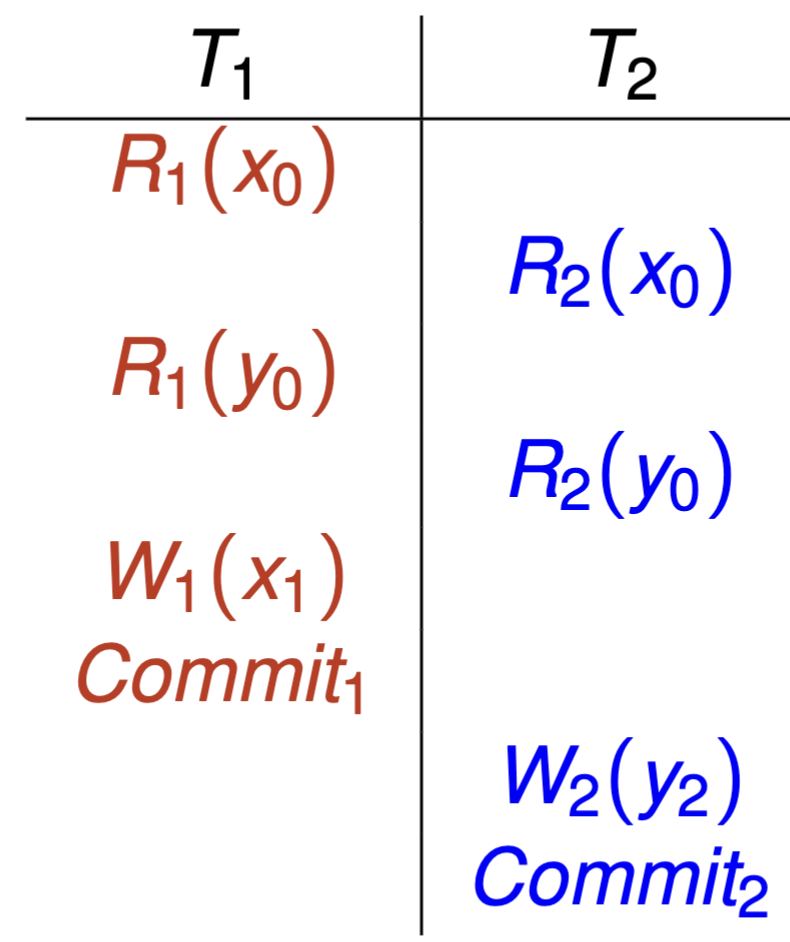
\includegraphics[width=0.2\linewidth]{cs3223-write-skew-anomaly.png} 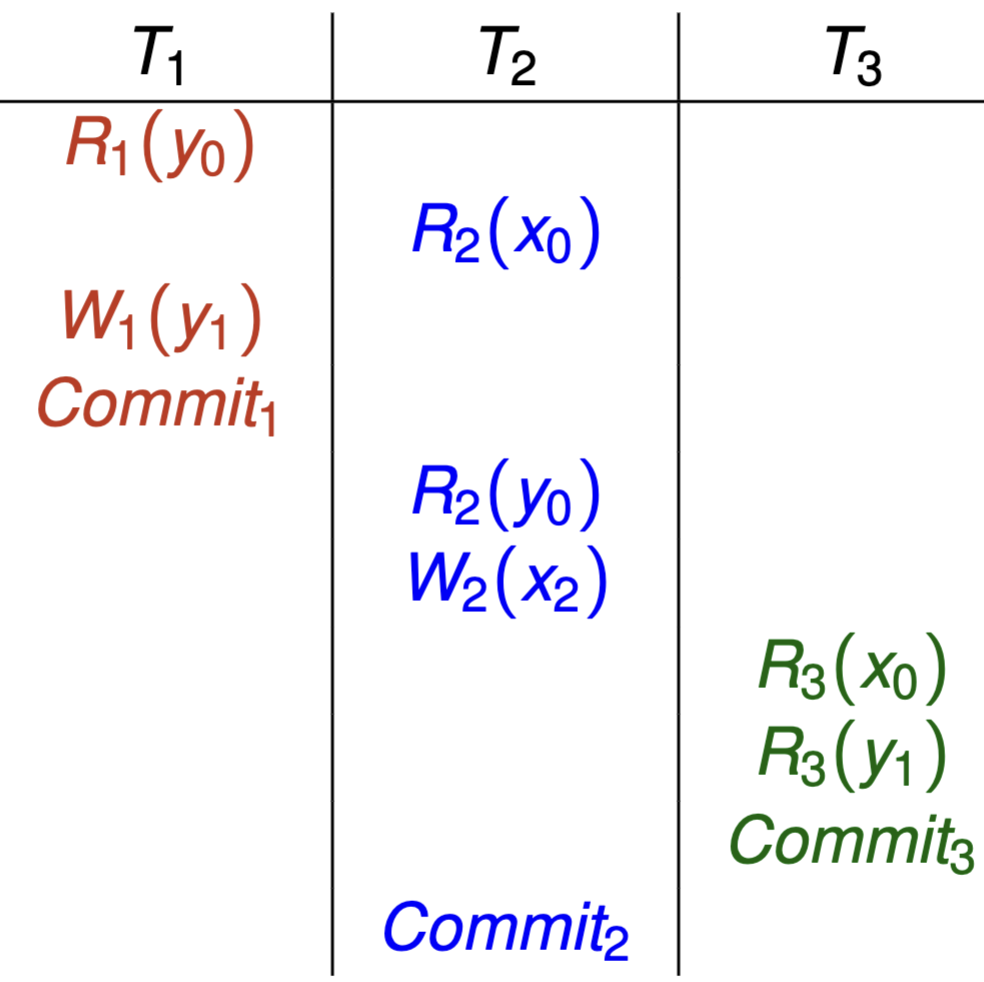
\includegraphics[width=0.25\linewidth]{cs3223-read-only-txn-anomaly.png} 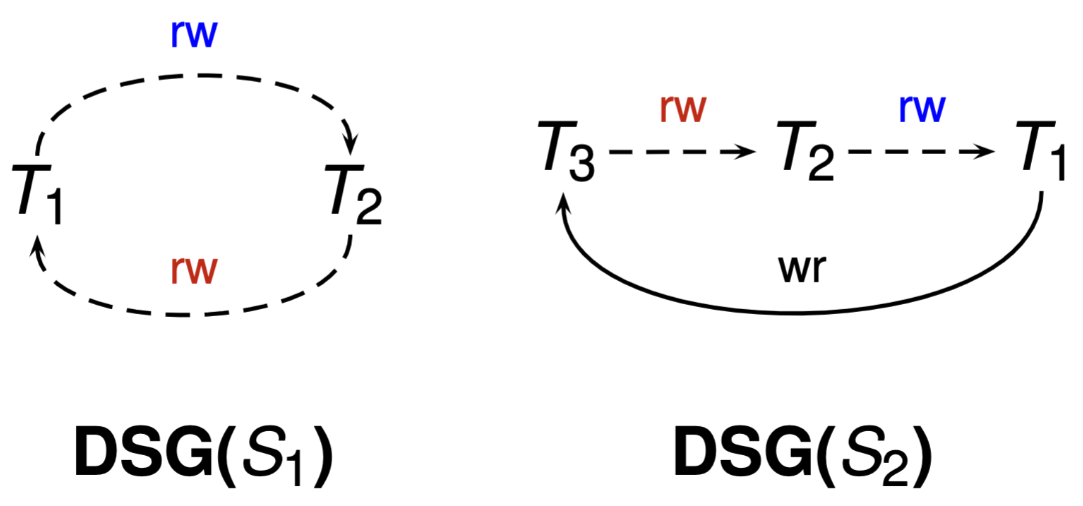
\includegraphics[width=0.4\linewidth]{cs3223-si-anomalies-revisited.png}

  \begin{itemize}
    \item \textbf{Serializable Snapshot Isolation (SSI)}: Guarantees serializable SI schedules.
    \item Transactional dependencies
    \begin{itemize}
      \item $T_1 \dashrightarrow_{ww} T_2$: $T_1$ writes a version of x. $T_2$ later writes \textbf{immediate successor} of x.
      \item $T_1 \dashrightarrow_{wr} T_2$: $T_1$ writes a version of x. $T_2$ later reads this version of x.
      \item $T_1 \dashrightarrow_{rw} T_2$: $T_1$ reads a version of x. $T_2$ later writes \textbf{immediate successor} of x.
      \item $x_j$ is the \textbf{immediate successor} of $x_i$ if $T_i$ commits before $T_j$ and no txn that commits between $T_i$'s and $T_j$'s commits produces x.
    \end{itemize}
    \item Maintain a Dependency Serializable Graph (DSG) to keep track of \textbf{rw dependencies} among concurrent T
    \item DSG(S) = (V, E), V = \{$T_1, \dots, T_k$\} and E
    \item $\dashrightarrow$ concurrent txn
    \item $\rightarrow$ non-concurrent txn
    \item If there exists a $T_j$ is involved in two rw concurrent dependencies, abort one of $T_i, T_j, T_k$.
    \item May result in unnecessary rollbacks due to false positives of SI anomalies.
    \item \textbf{Theorem Non-MVSS SI Schedules:} If S is a SI schedule that is \textbf{not MVSS}, then
    \begin{itemize}
      \item There is at least one cycle in DSG(S), and
      \item For each cycle in DSG(S), there exists three txns $T_i, T_j, T_k$ where
      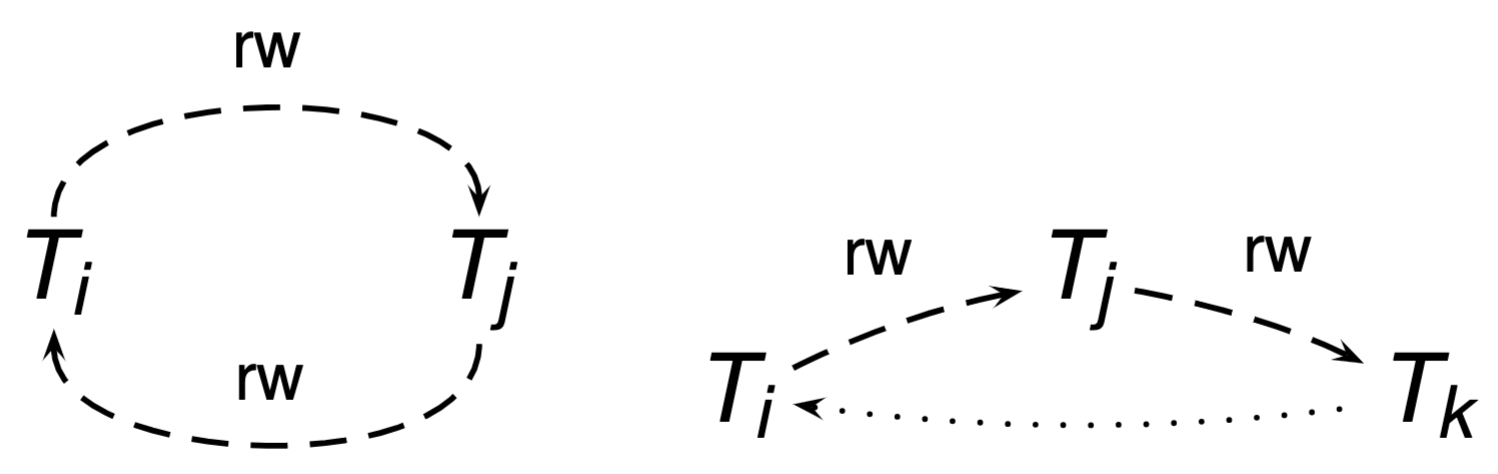
\includegraphics[width=0.1\textwidth]{cs3223-ssi-theorem.png}
    \end{itemize}
  \end{itemize}

  \subsection{10. Crash Recovery}
  \begin{itemize}
    \item Types of failure
    \begin{itemize}
      \item Transaction failure: T aborts
      \item System crash: loss of volatile memory contents
      \item Media failure: data is lost on non-volatile storage
    \end{itemize}
    \item \textbf{Recovery manager}: Supports Commit, Abort and Restart (abort all losers, and install updates from committed T not written to disk)
    \item desiderata: little overhead and recover quickly
    \item \textbf{Steal policy}: allow dirty pages updated by T to be replaced from buffer pool before T commits.
    \begin{itemize}
      \item No steal: poor throughput. Steal: how atomic?
    \end{itemize}
    \item \textbf{Force policy}: force dirty pages updated by T to written to disk when T commits
    \begin{itemize}
    
      \item poor response time but provide durability
    \end{itemize}
    \item 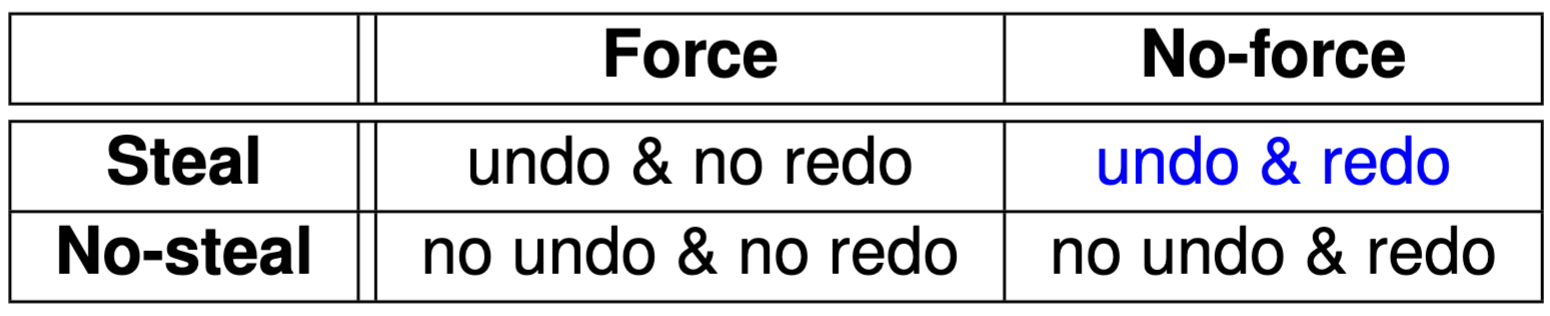
\includegraphics[width=0.12\textwidth]{cs3223-steal-force.png}
  \end{itemize}
\begin{itemize}
  \item 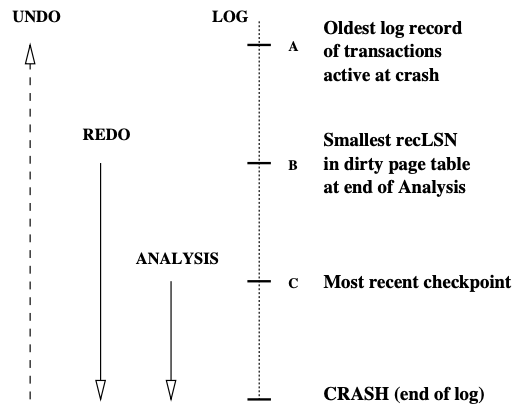
\includegraphics[scale=0.15]{cs3223-aries-three-phases.png}
  \item \textbf{Log} Sequential file of records in \textbf{non-volatile/stable storage} (multi copies)
  \begin{itemize}
    \item LSN: unique identifier, LSN of an earlier log record $<$ later log record
    \item type of log record (update, commit, abort)
    \item identifier of Xact
    \item pageID: what page is modified 
    \item prevLSN: LSN of the previous log record for same Xact
    \item undoNextLSN: See CLR
  \end{itemize}
  \item \textbf{Update log record}
  \begin{itemize}
    \item id of page being updated, byte offset within page indicating when updated portion start, length: number of byes for updated portion of page
    \item before-image and after-image of update
  \end{itemize}
  \item \textbf{Compensation Log Record (CLR)}
  \begin{itemize}
    \item When an update (described by a log record) is undone, create a CLR. Track action taken to undo update.
    \item undoNextLSN = LSN of next log record to be undone (this skips over the undone action in the LL) 
  \end{itemize}
  \item \textbf{Abort log record}: When Xact is to be aborted, start undoing this Xact.
  \item \textbf{End log record}: When the extra processing for aborted/committed Xact is done
  \item \textbf{Checkpoint log record}: See checkpointing
  \item \textbf{Transaction Table (TT)}
  \begin{itemize}
    \item One entry for each \textbf{active Txn} which contains
    \begin{itemize}
      \item XactID
      \item lastLSN: LSN of most \textbf{recent} log record for this Xact
      \item Xact status (C = committed or U = has not committed)
    \end{itemize}
  \end{itemize}
  \item \textbf{Dirty Page Table (DPT)}
  \begin{itemize}
    \item One entry for each \textbf{dirty page} in buffer pool which contains
    \begin{itemize}
      \item pageID: page ID of dirty page
      \item recLSN: LSN of the \textbf{earliest} log record for an update that dirtied page
    \end{itemize}
  \end{itemize}
  \item \textbf{Write-ahead logging (WAL) protocol}
  \item Uncommitted update to db not flushed til log with before-image is flushed.
  \item Each db page contains LSN of most recent log record (\textbf{pageLSN}) that describes update to the page. Before flushing db page p to disk, ensure that all log r' up to log r corresponding to p's pageLSN has been flushed.
  \item \textbf{Force-at-commit protocol}
  \item Do not commit a Xact until after-images of all its updated records are in stable storage (db or log). Enforced by writing a \textbf{commit log record} r for Xact and flushing all log records (up to and including r) for Xact to disk.
  \item An Xact is considered committed if its commit log is written to stable storage
  \item \textbf{Simple checkpointing}
  \item Stop accepting any new update, commit and abort ops.
  \item Wait till all active update, commit and abort ops are done.
  \item Flush all dirty pages in buffer.
  \item Write a checkpoint log record containing Xact table.
  \item Resume accepting new update, commit and abort.
  \item Analysis phase finds latest checkpoint log and resumes from there, init Xact to checkpoint and DPT to empty.
  \item \textbf{Fuzzy checkpointing}: Used by ARIES in analysis start up.
  \item Write begin checkpoint log record (BCPLR).
  \item Write end checkpoint log record (ECPLR) containing current DPT and TT.
  \item Write a master record containing LSN of begin checkpoint to stable storage.
  \item We assume there are no log records between BCPLR and ECPLR.
\end{itemize}

  \textbf{ARIES: Analysis}
  \begin{enumerate}
    \item Retrieve begin checkpoint log record (BCPLR) identified by master record
    \item Retrieve end checkpoint log record (ECPLR) corresponding to BCPLR
    \begin{itemize}
      \item We assume there are no log records between BCPLR and ECPLR
    \end{itemize}
    \item Initialize DPT and TT using ECPLR's contents
    \item Scan log record in forward direction to process each record r
    \item If r is an \textbf{end log record}
    \begin{itemize}
      \item Remove T from TT
    \end{itemize}
    \item Else
    \begin{itemize}
      \item Add an entry in TT for T if T is not in TT
      \item Update lastLSN of entry T to be r's LSN
      \item Update status of entry T to C if r is a commit log record
    \end{itemize}
    \item If (r is a redoable log record for page P) and (P is not in DPT) then
    \begin{itemize}
      \item Create entry for P in DPT with pageID = P's pageID, recLSN = r's LSN
    \end{itemize}
    \item At the end of Analysis, 1) TT = list of all active Txn at time of crash, 2) DPT = \textbf{superset} of dirty pages at time of crash
  \end{enumerate}

  \textbf{ARIES: Redo}
  \begin{enumerate}
    \item Set \textbf{RedoLSN} = smallest recLSN among all dirty pages in DPT
    \item Let $r$ be the log record with LSN = RedoLSN
    \item Scan the log in forward dir starting from $r$
    \item If (r is a \textbf{redoable} (update or CLR) log record) and (condition C is false)
    \begin{itemize}
      \item Fetch page P associated with r (this requires a page access!!!)
      \item If (P's pageLSN $<$ r's LSN) then
      \begin{itemize}
        \item Reapply logged action in r to P
        \item update P's pageLSN = r's LSN
      \end{itemize}
      \item Else
      \begin{itemize}
        \item Update P's entry in DPT: recLSN = P's pageLSN + 1
      \end{itemize}
    \end{itemize}
    \item At the end of Redo Phase, 1) Create \textbf{end log records} for Xacts with status = C in TT and remove them from TT, 2) System is restored to state at time of crash. (Still have losers)
    \item \textbf{Condition C}: (P is not in DPT) or (P's recLSN in DPT $>$ r's LSN)
  \end{enumerate}

  \textbf{ARIES: Undo}
  \begin{enumerate}
    \item Abort losers (active Xacts at time of crash) by undoing action in reverse order
    \item Initialize L = set of lastLSNs (with status = U) from TT
    \item Repeat until L becomes empty
    \begin{enumerate}
      \item Delete largest lastLSN from L
      \item Let r be the corresponding log record
      \item If r is an \textbf{update log record} for T on page P
      \begin{enumerate}
        \item Create a CLR $r_2$ for T: $r_2$'s undoNextLSN = r's prevLSN and prevLSN = T's lastLSN in TT
        \item Update T's entry in TT: lastLSN = $r_2$'s LSN
        \item Undo logged action on page P (WAL principle)
        \item update P's pageLSN = $r_2$'s LSN
        \item $Update-L-and-TT$(r's prevLSN) 
      \end{enumerate}
      \item else if r is a \textbf{CLR} for T then 
      \begin{enumerate}
        \item $Update-L-and-TT$(r's undoNextLSN)
      \end{enumerate} 
      \item else if r is an \textbf{abort log record}
      \begin{enumerate}
        \item $Update-L-and-TT$(r's prevLSN)
      \end{enumerate}
      \item \textbf{def} $Update-L-and-TT$(lsn)
      \begin{enumerate}
        \item if lsn is not null then add lsn to L
        \item else create an \textbf{end log record} for T and remove T from TT
      \end{enumerate}
    \end{enumerate}
  \end{enumerate}

\end{multicols*}

\end{document}
